\chapter{Design}
\label{ch:design}

\section{Threat Model}
\label{sec:threat-model}

In this threat model, we differentiate between two aspects of memory safety:

\begin{figure}
    \centering
    \begin{subfigure}[T]{0.45\textwidth}
        \centering
        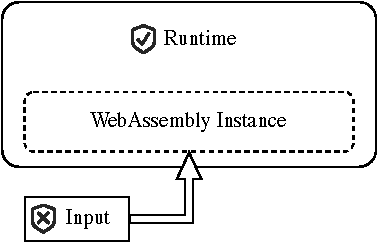
\includegraphics{figures/build/wasm-internal-mem-safety}
        \caption{Internal Memory Safety}
        \label{fig:internal-mem-safety}
    \end{subfigure}
    \hfill
    \begin{subfigure}[T]{0.45\textwidth}
        \centering
        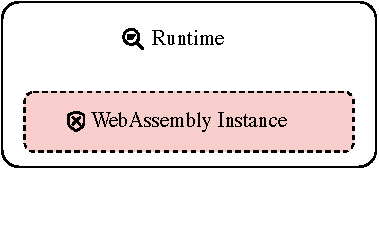
\includegraphics{figures/build/wasm-external-mem-safety}
        \caption{External Memory Safety}
        \label{fig:external-mem-safety}
    \end{subfigure}
    \caption{Threat model for internal and external memory safety}
    \label{fig:threat-model}
\end{figure}

\begin{description}
    \item[Internal Memory Safety]: Ensures memory safety within the boundaries of a sandbox.
    Our point of view is from within a WebAssembly instance, we trust the runtime (and the host we are running on), but we do not trust external input.
    See \cref{fig:internal-mem-safety}
    \item[External Memory Safety]: Maintains the memory safety of the sandbox itself against potentially malicious programs.
    Our point of view is from the runtime, we trust the platform we're running on, but not the WebAssembly programs we are executing.
    See \cref{fig:external-mem-safety}
\end{description}

\subsection{Internal Memory Safety}
\label{subsec:internal-memory-safety}
For internal memory safety, the program within the sandbox and its runtime, including its compiler, are considered trusted and assumed to be free of bugs.
Untrusted input (e.g., network data, file reads) originates from outside the sandbox and may be controlled by an attacker.
This model mirrors the threat environment of a standard non-\ac{WASM} program.
Potential threats include:

\begin{itemize}
    \item \textbf{Buffer overflows} Attempts to write data beyond allocated buffer boundaries.
    \item \textbf{Use-after-free} Accessing memory after it has been deallocated.
\end{itemize}

As discussed in \cref{sec:wasm}, WebAssembly's design inherently mitigates certain threats common in non-\ac{WASM} environments, so we will not consider the following vectors:

\begin{itemize}
    \item \textbf{Return-oriented attacks} {\ac{WASM}'s} structured control flow constructs prevent arbitrary code execution through stack manipulation.
    \item \textbf{Calling unknown function pointers} Function tables enforce a strict mechanism for function calls, ensuring the integrity of call targets.
\end{itemize}

\subsection{External Memory Safety}
\label{subsec:external-memory-safety}

For external memory safety, we focus on the security of the sandbox.
Threats originate from running untrusted programs, which may be buggy or adversarial.

\begin{itemize}
    \item \textbf{Sandbox escapes}: Attempts to break out of the sandbox's restrictions and access host resources.
    \item \textbf{Side-channel attacks}: Exploiting timing differences or resource usage patterns to infer sensitive information.
\end{itemize}

We assume that the operating system and underlying target architecture is free of bugs that might be exploited by malicious targets.
This does not include assumptions about potential spectre-like~\cite{kocher2020spectre} attacks.
The compiler needs to ensure bounds checks are guarded against side-channel attacks.

Additionally, we do not consider exploits of the program running in the sandbox as vulnerabilities.
As far as the runtime is concerned, as long as exploits are contained within the sandbox, the security objectives have been met.

\section{Overview}
\label{sec:overview}

\begin{figure*}[t]
    \centering
    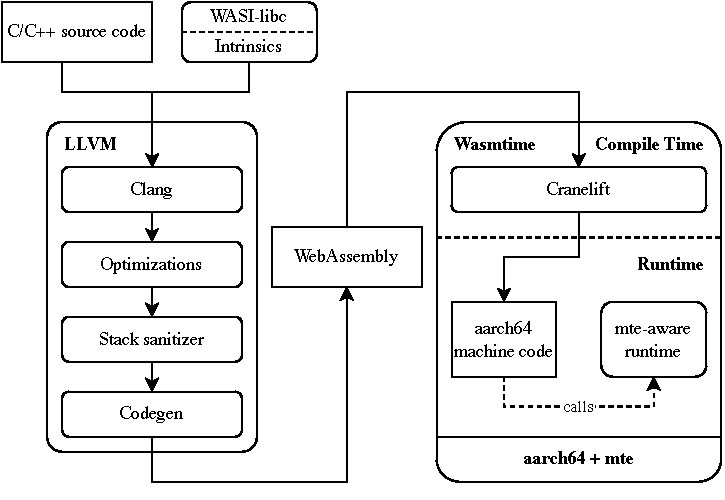
\includegraphics{figures/build/overview}
    \caption{Overview of the adapted workflow}
    \label{fig:overview}
\end{figure*}

% TODO: these figures don't quite fit here. Move them somewhere it makes sense. Maybe implementation?
\begin{figure}[t]
    \centering
    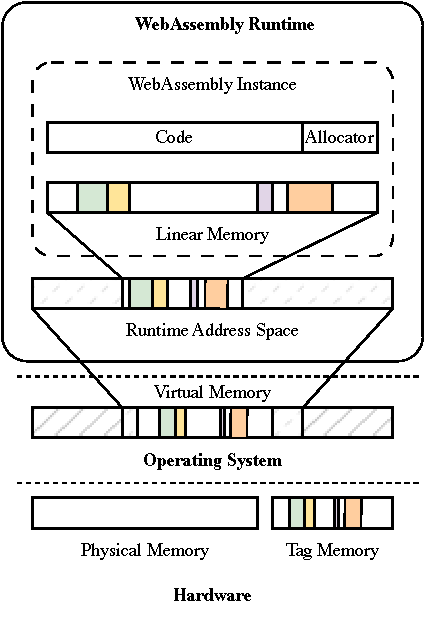
\includegraphics[scale=1]{figures/build/system-design-2}
    \caption{System Design of our Memory Safety Extension.}
    \label{fig:system-design-2}
\end{figure}

Figure~\ref{fig:overview} presents an overview of \projectname{}.

At build time, the unmodified C/C++ sources, along with a modified version of libc, are compiled using LLVM~\cite{lattner2004llvm}.
After optimizations, a stack sanitizer analyzes all functions, and inserts instrumentation as necessary.
LLVM's backend then generates WebAssembly binaries that can be deployed and executed on a multitude of devices.

\section{WebAssembly Extension}
\label{sec:wasm-extension}

We designed an extension to WebAssembly that provides primitives to the modified standard library and the stack sanitizer to guarantee memory safety for selected allocations.
Our extension builds on top of wasm64, the 64\,bit variant of WebAssembly.
We chose wasm64, as wasm64 uses a 64\,bit integer index type, with 48 of those bits being used to index memory.
This allows utilizing 16 bits for metadata about the allocation.

For our extension, we introduce the notion of abstract segments and tagged pointers.
We introduce three new instructions that allow creating abstract segments and tagged pointers from raw pointers.
These pointers carry provenance with them and can only access the segment they were created with.
Conversely, segments can only be accessed by the tagged pointer created with them and not with raw indices without provenance.
The instructions are type-checked according to \cref{fig:typing-rules}.

\begin{equation*}
    \text{(new instructions) } e \Coloneqq \textbf{segment.new} \mid \textbf{segment.set\_tag} \mid \textbf{segment.free}
\end{equation*}


\begin{figure}[t]
    \begin{prooftree}
        \AxiomC{$C_{\text{memory}} = n$}
        \AxiomC{$2^a=16$}
        \BinaryInfC{$C \vdash \textbf{segment.new}\ a\ o : \text{i64}\ \text{i64} \rightarrow \text{i64}$}
    \end{prooftree}
    \begin{prooftree}
        \AxiomC{$C_{\text{memory}} = n$}
        \AxiomC{$2^a=16$}
        \BinaryInfC{$C \vdash \textbf{segment.set\_tag}\ a\ o : \text{i64}\ \text{i64}\ \text{i64} \rightarrow \epsilon$}
    \end{prooftree}
    \begin{prooftree}
        \AxiomC{$C_{\text{memory}} = n$}
        \AxiomC{$2^a=16$}
        \BinaryInfC{$C \vdash \textbf{segment.free}\ a\ o : \text{i64}\ \text{i64} \rightarrow \epsilon$}
    \end{prooftree}
    \caption{Typing rules}
    \label{fig:typing-rules}
\end{figure}

\paragraph{}
Following, we will describe the new instructions in detail.

\begin{description}
    \item[\texttt{segment.new}] Create a new, zeroed memory segment.
    This instruction takes two parameters, a memory index and a size.
    The instruction generates a new tag, assigns it to the piece of memory, and returns a tagged pointer that can be used to access the segment.
    \item[\texttt{segment.set\_tag}] Takes a memory index, a length and a tagged pointer and applies the tag from the tagged pointer to the memory segment located at the index with the passed length.
    This can be used to move ownership from one segment to another, or to merge segments.
    \item[\texttt{segment.free}] Invalidates a segment by reassigning a new, implementation defined tag.
    This instruction takes two parameters, a memory index and a length.
    After this instruction, the tagged pointer being used to access the segment is no longer valid, and accessing the segment through it will result in a trap.
\end{description}

We also modify the semantics of existing load and store instructions.
They still take an integer as an index, but we introduce provenance to integers, which is tracked using the unused 16 upper bits in pointers.
Untagged indices may be used to access memory that has not been claimed as a segment.
If a segment is accessed, the runtime will check that the tagged pointer is allowed to access the segment, i.e.\ the index is the index returned by the \texttt{segment.new} instruction.
If this is not the case, a trap is thrown.

This has the important consequence that unmodified code will continue working as-is, as load and store instructions will transparently handle both tagged and untagged indices.
This design choice allows the gradual integration of safety primitives into specific parts of WebAssembly applications where enhanced security is required.
For instance, it enables the introduction of a customized malloc implementation, which prevents spatial and temporal safety bugs for heap-allocated memory.
Stack accesses can be analyzed to instrument only accesses that are accessed using untrusted offsets or have their address taken, while stack slots that are simply register spills or scalar values do not have to be instrumented, improving performance.

\paragraph{Alignment}
All segments are aligned to 16 bytes, which corresponds to the alignment of MTE (see \cref{subsec:mte}).
This is an implementation choice, that can and will be changed once we support additional implementations.
More detail can be found in \cref{sec:future-work}.

\subsection{Example}
\label{subsec:example}

We will demonstrate our \ac{WASM} extension using the following C snippet, which allocates 64 bytes on the stack.
This requires the compiler to instrument the stack allocation, creating a new segment, and freeing the segment before returning to the caller, i.e. tagging the stack slot with the stack frame's tag.

\begin{lstlisting}[frame=h,style=customc,
    label={lst:wasm-example-c}]
void foo() {
    char buf[64];
    // ...
    return;
}
\end{lstlisting}

When compiling to \ac{WASM}, the compiler allocates the slot on the stack, decrementing the global \lstinline[style=customwasm]{$__stack_pointer} acting as the stack pointer.
Then, a new segment of size 64 is created and the tagged pointer to it is stored in the local \lstinline[style=customwasm]{$buf}.
Before returning, the segment is retagged using the stack pointers tag, i.e. restoring the previous tag and allowing access through the stack pointer.
Then, the stack pointer is reset, freeing the stack frame.

\begin{lstlisting}[frame=h,style=customwasm,
    label={lst:wasm-example}]
;; Allocate space on the stack
global.get $__stack_pointer
i64.const 64
i64.sub
global.tee $__stack_pointer

;; tag the segment
i64.const 64
segment.new
local.set $buf

;; ...

;; retag with stack pointer tag
local.get $buf
global.get $__stack_pointer
i64.const 64
segment.set_tag

;; reset stack pointer
global.get $__stack_pointer
i64.const 64
i64.sub
global.set $__stack_pointer
\end{lstlisting}

\subsection{Heap Safety}
\label{subsec:heap-safety}

To provide heap safety, the memory allocator needs to be aware of segments.
When allocating memory, the requested size is aligned to 16 bytes, and a segment is returned to the caller.
This prevents overflows from corrupting allocator metadata or other memory segments.

\subsection{Stack Safety}
\label{subsec:stack-safety}

For stack safety, we create segments from stack slots when entering a function.
Before returning, all stack slots are untagged and reassigned to the stack frame.
This not only allows other functions to use the memory, but also prevents stack slots from being accessed after returning from a function.

However, not every stack slot needs to be turned into a segment, e.g.\ register spill slots, stack slots that do not escape, or stack slots that never have their address taken.
Creating segments for these would create excessive runtime and memory overhead, as each stack slot would need to be aligned to 16 bytes and processed when entering and returning from a function.

To address this, we designed an algorithm that identifies safe memory regions within the stack that do not require protection, thus avoiding creating segments for the aforementioned slots.
Below we present a simplified version of our algorithm.
We iterate over all stack allocations and check if the allocation (a) escapes the function or (b) is indexed into using an unsafe \ac{GEP} instruction.

\begin{algorithmic}
    \State $allocsToInstrument \gets \emptyset$
    \For{$alloc \in allocations$}
        \If{escapes($alloc$)}
            \State $allocsToInstrument$.push($alloc$)
        \EndIf
        \If{isUsedByUnsafeGEP($alloc$)}
            \State $allocsToInstrument$.push($alloc$)
        \EndIf
    \EndFor

    \For{$alloc \in allocsToInstrument$}
        \State insertTaggingCode($alloc$)
        \State insertUntaggingCode($alloc$)
    \EndFor
\end{algorithmic}

\subsection{Example}
\label{subsec:example2}

We demonstrate the algorithm using the following function.

\begin{lstlisting}[frame=h,style=customc,
    label={lst:stack-safety}]
char foo(int index) {
  int i = 0; // safe
  int bytes_read = 0; // unsafe
  char buf[32]; // unsafe
  read_input(buf, &bytes_read);
  return buf[index];
}

char *bar() {
    char buf[32]; // unsafe
    return buf;
}
\end{lstlisting}

In the code example above, \texttt{i} is safe, as its address is not used in a potentially unsafe address computation and does not escape.
The variables \texttt{bytes\_read} and \texttt{buf} are determined to be unsafe, as their address escapes.
Additionally, \texttt{buf} is accessed using an untrusted index.

In function \texttt{bar}, \texttt{buf} also needs to be instrumented, as it again escapes.
Any attempt to use the value returned by \texttt{bar} is undefined behavior and will be caught by our instrumentation, preventing difficult to debug bugs or potential vulnerabilities.

\noindent
Our algorithm effectively balances the need for stack safety with performance and memory efficiency constraints.

\section{Hardware-Assisted Sandboxing}
\label{sec:bounds-checks}

WebAssembly runtimes ensure that applications remain within their allocated memory sandbox.
This is traditionally achieved through bounds checks or by leveraging the operating system's virtual memory management.
In wasm32, runtimes typically employ memory-mapping techniques, statically mapping the entire 32\,bit addressable space and marking unpermitted areas as inaccessible.
Accessing these inaccessible pages results in a segmentation fault, which is caught by the runtime, effectively containing the guest code within its sandbox.

However, this strategy faces limitations in wasm64 due to the impracticality of mapping the entire 64-bit address space.
This constraint necessitates the insertion of bounds checks, which can significantly degrade performance.
% TODO: make sure the impact is actually shown.
We demonstrate the impact of these checks on wasm64 execution speed in section~\ref{ch:eval}.

In \cref{fig:system-design-sandboxing}, we showcase an approach that utilizes memory tagging to replace software-based bounds checls.
On module instantiation, the runtime assigns a random tag to the linear memory and the heap base address.
Memory access translation then involves adding this tagged heap base address to the accessed index.

\begin{figure}[t]
    \centering
    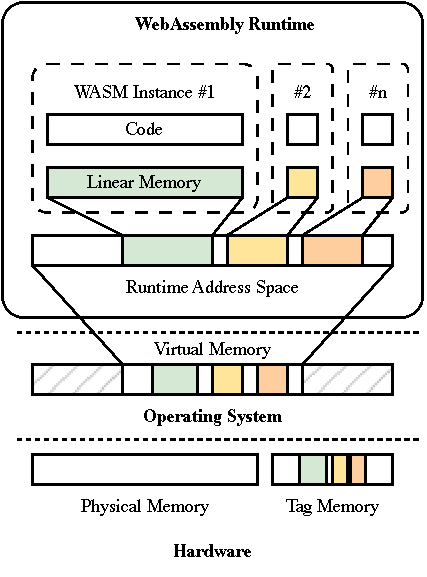
\includegraphics[scale=1]{figures/build/system-design-1}
    \caption{Bounds checks are replaced with MTE}
    \label{fig:system-design-sandboxing}
\end{figure}

However, we face a limitation in the number of sandboxes for this approach.
Since \ac{MTE} only offers up to 16 distinct tags, we are limited to at most 15 different sandboxes within one process, as we need to reserve one tag for the runtime.

\subsection{Combining memory safety with MTE bounds checks}
\label{subsec:combining-memory-safety-with-mte-bounds-checks}

If we combine this sandboxing approach with our \ac{MTE}-backed \ac{WASM} extension, we need to ensure malicious programs cannot break out of the sandbox by forging or manipulating tags, while still retaining the performance benefit of \ac{MTE}-based sandboxing.

There is two challenges we need to take care of:
\begin{enumerate}
    \item Adding a tagged user pointer to the heap base address should be performant and result in the correct tag for the respective memory.
    \item It's crucial to prevent users from creating tags that enable access beyond their allocated memory sandbox.
\end{enumerate}

We designate the lowest tag bit to determine whether memory belongs to the runtime or to the linear memory.
Memory belonging to the runtime is tagged with the zero tag, while the linear memory is initially tagged with the tag 1.
The remaining three tag bits are used for the memory safety features and can be generated by \texttt{segment.new}.
This results in memory indices always being tagged with an even tag, but once we actually access memory, we do so with an odd tag.

When tagging memory using these primitives, we set the lowest tag bit to 1 before tagging.

\begin{lstlisting}[frame=h,style=customc,
    label={lst:generated-code-tagging}]
// tagging memory
v0 = or tag, 0x0100_0000_0000_0000
stzg v0, [address]
\end{lstlisting}

Memory accesses are translated by adding the tagged heap base to the tagged index, as can be seen in \cref{fig:system-design-mem-safety-bounds}.

\begin{figure}[t]
    \centering
    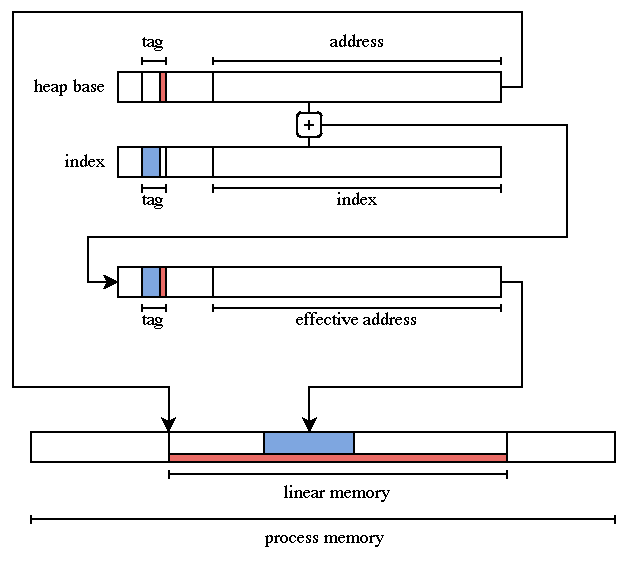
\includegraphics[scale=0.75]{figures/build/bounds-mem-safety}
    \caption{MTE-based bounds checks}
    \label{fig:system-design-mem-safety-bounds}
\end{figure}

However, since the memory index is untrusted, an attacker may craft a value that overflows the tag bits when adding it to the heap base, resulting in a tag that allows accessing memory outside the linear memory.
To prevent this, we need to set the lowest tag bit via a bitwise mask before each memory access, as can be seen below.

\begin{lstlisting}[frame=h,style=customc,
    label={lst:generated-code-mem-access}]
// accessing memory
v0 = add heap_base, index
v1 = or v1, 0x0100_0000_0000_0000
\end{lstlisting}

With this approach, we prevent attempts by untrusted code to access runtime memory through forged tags.

